\documentclass[letterpaper, 12pt]{article}
\usepackage[utf8]{inputenc}
\usepackage[margin=1.0in]{geometry}
\usepackage{mathtools}
\usepackage{listings}
\usepackage{xcolor}
\usepackage{blindtext}
\usepackage{enumitem}
\usepackage{caption}
\usepackage{tgschola}
\usepackage{textcomp}
% NFA
\usepackage{tikz}
\usetikzlibrary{automata, positioning, arrows}

%%%%% C Code Style %%%%%
\definecolor{comment}{RGB}{0,128,0} % dark green
\definecolor{string}{RGB}{255,0,0}  % red
\definecolor{keyword}{RGB}{0,0,255} % blue

\lstdefinestyle{c}{
	commentstyle=\color{comment},
	stringstyle=\color{string},
	keywordstyle=\color{keyword},
	basicstyle=\footnotesize\ttfamily,
	numbers=left,
	numberstyle=\tiny,
	numbersep=5pt,
	frame=lines,
	breaklines=true,
	prebreak=\raisebox{0ex}[0ex][0ex]{\ensuremath{\hookleftarrow}},
	showstringspaces=false,
	upquote=true,
	tabsize=3,
}
%%%%% C Code Style %%%%%

\title{CS416 Operating Systems Design\\Homework 0: Skills Survey}
\author{William Chen}
\date{January 16, 2018}

\begin{document}

\section*{Questions}

\begin{itemize}
	\item [0.] Predict the output of this snippet:

\begin{lstlisting}[language=C, style=c]
int main() {
	int main = 56;
	printf("%d", main);
	return 0;
}
\end{lstlisting}

	\begin{enumerate}[label=(\alph*)]
		\item Compiler Error
		\item Depends on the compiler
		\item 56	$\leftarrow$
		\item none of the above
	\end{enumerate}

	\item [1.] Predict the output of this snippet:

\begin{lstlisting}[language=C, style=c]
#include <stdio.h>
int main() {
	char ch;
	if (ch = printf("")) {
		printf("It matters\n");
	}
	else {
		printf("It doesn't matter\n");
	}
	return 0;
}
\end{lstlisting}

	\begin{enumerate}[label=(\alph*)]
		\item It matters
		\item It doesn't matter	$\leftarrow$
		\item Runtime error
		\item Nothing
	\end{enumerate}


	\item[2.] How many times is Hello world printed by the code snippet below?

\begin{lstlisting}[language=C, style=c]
int main() {
	fork();
	fork();
	printf("Hello world\n");
}
\end{lstlisting}

	\begin{enumerate}[label=(\alph*)]
		\item 1
		\item 2
		\item 4	$\leftarrow$
		\item 8
	\end{enumerate}

	\item[3.] What is the output of this C code?

\begin{lstlisting}[language=C, style=c]
#include <stdio.h>
int main() {
	int x = 1, y = 0, z = 5;
	int a = x && y || ++z;
	printf("%d", z++);
}
\end{lstlisting}

	\begin{enumerate}[label=(\alph*)]
		\item 1
		\item 5
		\item 6	$\leftarrow$
		\item 7
	\end{enumerate}

	\item[4.] What is the output of this C code?

\begin{lstlisting}[language=C, style=c]
#include <stdio.h>
int main() {
	int y = 2;
	int z = y +(y = 10);
	printf("%d\n", z);
}
\end{lstlisting}

	\begin{enumerate}[label=(\alph*)]
		\item 2
		\item 4
		\item 20	$\leftarrow$
		\item Compile time error
	\end{enumerate}

	\item[5.] What is the output of this C code?

\begin{lstlisting}[language=C, style=c]
#define max(a) a
int main() {
	int x = 1;
	switch (x)
	{
		case max(2):
			printf("yes\n");
		case max(1):
			printf("no\n");
		break;
	}
}
\end{lstlisting}

	\begin{enumerate}[label=(\alph*)]
		\item yes
		\item no $\leftarrow$
		\item Runtime error
		\item Compile time error
	\end{enumerate}

	\item[6.] What is the output of this C code?

\begin{lstlisting}[language=C, style=c]
#include <stdio.h>
int main() {
	int x = 35;
	printf("%d %d %d", x == 35, x = 50, x > 40);
	return 0;
}
\end{lstlisting}

	\begin{enumerate}[label=(\alph*)]
		\item 1 50 1
		\item 0 50 0	$\leftarrow$
		\item Runtime error
		\item Compile time error
	\end{enumerate}

	\item[7.] You have two numbers, A and B.

	Using bitwise operations and loops, write code to determine how many bits must be flipped in order to turn A in to B.

	e.g.

	A: 101001

	B: 10\textbf{01}01

	Answer: 2 bits\\

\begin{lstlisting}[language=C, style=c]
int flipBits (int a, int b) {
	unsigned int count = 0;
	unsigned int i = a ^ b;
	while (i != 0) {
		int j = i & 1;	// 0b00000000000000000000000000000001
		i = i >> 1;
		if (j != 0) {
			count++;
		}
	}
	return count;
}
\end{lstlisting}

	\item[8.] Presume you have an implementation of Quick-sort that picks the first element in a list as its pivot.

	Construct a list of 13 numbers that would make this algorithm run in $O(n^2)$ time.

	Solution: $1, 2, 3, 4, 5, 6, 7, 8, 9, 10, 11, 12, 13$

	\item[9.] Write code to solve the below in $O(n)$ time with one pass over the array. If you can not, provide your best code and state the asymptotic running time.

	In this challenge, given an array of integers, the goal is to efficiently find the subarray that has the greatest positive value when all of its elements are summed together.

	Write some code that, if given an array of integers, will find the subarray that has the greatest sum. A subarray is a contiguous subset of the original array.

	Keep in mind the maximal subarray is not necessary a proper subset, and might contain the whole original array.

	Be careful. Some array elements may be negative, so less can be more.

	If all the elements in an array are negative, the maximal sum should be null as we are interested in the greatest positive value, not the greatest arithmetic value.

	For example, given the array: $\left\{1, 2, -5, 4, -3, 2\right\}$
	\begin{itemize}
		\item The maximum sum of a subarray is 4 and it contains only the element 4.
	\end{itemize}

	Before you write the code, take some time to think of the most efficient solution possible; it may surprise you. The major goal of this question is to test your algorithmic skills rather than merely your ability to write code quickly.\\

\begin{lstlisting}[language=C, style=c]
int maxSubarray(int* array, int len, int** pArrayOut, int* pLenOut) {
	// Max subarray so far
	int 	sumMax 		= 0;
	int 	startIdxMax = 0;
	int 	lenMax 		= 0;
	// Max of subarray end at Index
	int 	sumMaxEndHere		= 0;
	int 	startIdxMaxEndHere  = 0;
	int 	lenMaxEndHere		= 0;

	int i;
	for (i=0; i < len; i++) {
		// Find sumMaxEnd at this Index
		if (sumMaxEndHere > 0) {
			sumMaxEndHere		= sumMaxEndHere + *(array+i);
			//startIdxMaxEndHere = startIdxMaxEndHere;
			lenMaxEndHere			= lenMaxEndHere + 1;
		}
		else {
			sumMaxEndHere		= *(array+i);
			startIdxMaxEndHere 	= i;
			lenMaxEndHere		= 1;
		}
		if (sumMaxEndHere > sumMax) {
			sumMax 		= sumMaxEndHere;
			startIdxMax = startIdxMaxEndHere;
			lenMax 		= lenMaxEndHere;
		}
	}
	if (pArrayOut) {
		*pArrayOut = array + startIdxMax;
	}
	if (pLenOut) {
		*pLenOut = lenMax;
	}
	return sumMax;
}
\end{lstlisting}


	\item[10.] RE pattern matching.\\
	Draw an NFA (nondeterministic finite state automaton)
	that recognizes the same language that the regular expression $((A^*B | C )^* | D )$

	% NFA
	\begin{figure}[h]
		\centering
		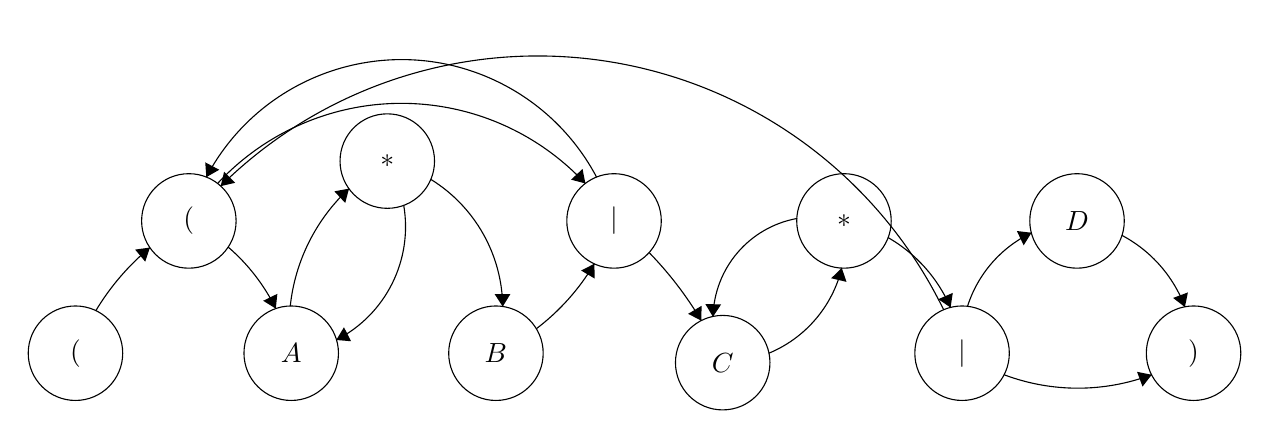
\begin{tikzpicture}[scale=0.2]
			\tikzstyle{every node}+=[inner sep=0pt]
			\draw [black] (3.2,-42.1) circle (3);
			\draw (3.2,-42.1) node {$($};
			\draw [black] (16.9,-42.1) circle (3);
			\draw (16.9,-42.1) node {$A$};
			\draw [black] (23,-29.9) circle (3);
			\draw (23,-29.9) node {$*$};
			\draw [black] (29.9,-42.1) circle (3);
			\draw (29.9,-42.1) node {$B$};
			\draw [black] (37.4,-33.7) circle (3);
			\draw (37.4,-33.7) node {$|$};
			\draw [black] (44.3,-42.7) circle (3);
			\draw (44.3,-42.7) node {$C$};
			\draw [black] (52,-33.7) circle (3);
			\draw (52,-33.7) node {$*$};
			\draw [black] (59.5,-42.1) circle (3);
			\draw (59.5,-42.1) node {$|$};
			\draw [black] (66.8,-33.7) circle (3);
			\draw (66.8,-33.7) node {$D$};
			\draw [black] (74.2,-42.1) circle (3);
			\draw (74.2,-42.1) node {$)$};
			\draw [black] (10.4,-33.7) circle (3);
			\draw (10.4,-33.7) node {$($};
			\draw [black] (16.839,-39.109) arc (-186.05342:-227.07669:11.905);
			\fill [black] (20.57,-31.65) -- (19.64,-31.82) -- (20.33,-32.56);
			\draw [black] (11.51,-30.919) arc (152.11727:27.88273:14.018);
			\fill [black] (11.51,-30.92) -- (12.33,-30.45) -- (11.44,-29.98);
			\draw [black] (25.756,-31.055) arc (58.34161:0.64112:9.629);
			\fill [black] (30.33,-39.14) -- (30.82,-38.34) -- (29.82,-38.35);
			\draw [black] (12.224,-31.323) arc (137.1087:42.8913:15.937);
			\fill [black] (35.58,-31.32) -- (35.4,-30.4) -- (34.67,-31.08);
			\draw [black] (12.421,-31.485) arc (134.61693:25.96678:28.667);
			\fill [black] (12.42,-31.49) -- (13.34,-31.28) -- (12.64,-30.57);
			\draw [black] (24.042,-32.695) arc (9.80487:-62.93498:8.072);
			\fill [black] (19.76,-41.26) -- (20.7,-41.34) -- (20.25,-40.45);
			\draw [black] (51.863,-36.679) arc (-13.56603:-67.53163:7.867);
			\fill [black] (51.86,-36.68) -- (51.19,-37.34) -- (52.16,-37.57);
			\draw [black] (43.684,-39.791) arc (-181.27155:-259.8261:6.496);
			\fill [black] (43.68,-39.79) -- (44.2,-39) -- (43.2,-38.98);
			\draw [black] (36.147,-36.42) arc (-30.69301:-52.82759:14.415);
			\fill [black] (36.15,-36.42) -- (35.31,-36.85) -- (36.17,-37.36);
			\draw [black] (4.493,-39.398) arc (148.99416:129.80325:15.829);
			\fill [black] (7.93,-35.39) -- (6.99,-35.52) -- (7.63,-36.29);
			\draw [black] (12.892,-35.357) arc (49.3789:26.08719:12.262);
			\fill [black] (15.92,-39.27) -- (16.02,-38.33) -- (15.12,-38.77);
			\draw [black] (54.795,-34.754) arc (60.21251:23.30809:9.423);
			\fill [black] (58.77,-39.2) -- (58.91,-38.27) -- (57.99,-38.67);
			\draw [black] (59.84,-39.138) arc (-197.55825:-244.42615:7.809);
			\fill [black] (63.91,-34.45) -- (62.98,-34.34) -- (63.41,-35.25);
			\draw [black] (69.642,-34.612) arc (62.15464:20.60239:8.554);
			\fill [black] (73.65,-39.17) -- (73.84,-38.24) -- (72.9,-38.59);
			\draw [black] (71.536,-43.466) arc (-69.3217:-110.6783:13.271);
			\fill [black] (71.54,-43.47) -- (70.61,-43.28) -- (70.96,-44.22);
			\draw [black] (39.626,-35.708) arc (44.23934:30.71302:23.117);
			\fill [black] (42.94,-40.03) -- (42.96,-39.09) -- (42.1,-39.6);
		\end{tikzpicture}
		\caption*{NFA for $((A^*B | C )^* | D )$}
	\end{figure}

\end{itemize}

\end{document}